En este primer paso se busca familiarizarse con los datos y series de tiempo que se tienen, respecto al tipo de cambio entre la libra esterlina y el dólar (GBP-USD). Con este motivo, se pide buscar los hechos históricos importantes en el período de estudio que afectaron a los mercados involucrados y el tipo de cambio en juego. A continuación se presenta la variación del tipo de cambio en el transcurso de Enero del año 2016 a Enero del año 2019:

\begin{figure}[H]
    \begin{center}
    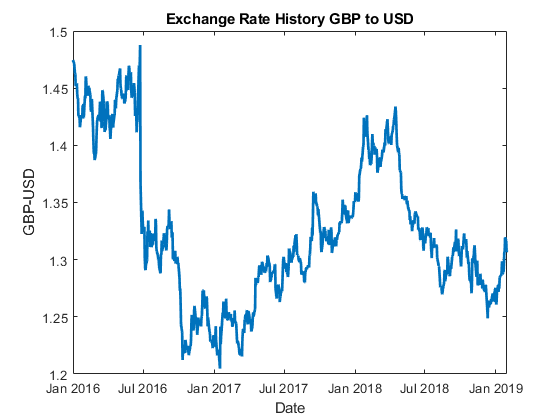
\includegraphics[width = 13cm]{figures/data.png}
    \caption{Tipo de cambio GBP-USD entre año 2016 y 2019}
    \label{fig:my_label1} %El label permite citar el gráfico, pero es para más adelante
    \end{center}
\end{figure}
\newpage

\noindent En el gráfico anterior se pueden observar diversos tramos en los cuales el tipo de cambio fluctúa, encontrándose la libra esterlina más depreciada o apreciada respecto al dólar. De manera general, estas fluctuaron acorde al proceso de separación que estaba llevando el Reino Unido para dejar de formar parte de la Unión Europea, proceso comúnmente denominado como \textit{Brexit}, lo que se reflejó en una inestabilidad del valor de la libra esterlina durante dicho período. Finalmente, dentro de los hechos históricos importantes acontecidos durante este período tenemos los siguientes:

\begin{itemize}
    \item Febrero 2016: El alcalde de Londres, Boris Johnson, le otorgó todo su apoyo y voto al \textit{Brexit}, lo que provocó que los inversores vieran un mayor riesgo en el país, que finalmente se tradujo en un retiro de fondos por parte de los inversionistas y por ende una depreciación de la libra esterlina.
    
    \item Junio 2016: El referéndum celebrado el 23 de Junio de 2016, con motivo del \textit{Brexit}, presentó una aprobación equivalente al 51,9\% de los votantes apoyando la idea de abandonar la \textit{Unión Europea}, por lo cual se procedió a invocar el artículo 50 del \textit{Tratado de la Unión Europea}, con lo que, nuevamente se vieron reflejados los problemas y preocupaciones asociadas a la salida del \textit{Reino Unido} de la \textit{Unión Europea}, provocando nuevamente un retiro de capitales.
    
    \item Febrero 2017: Desde este periodo, hasta comienzos del año 2018, se pudo observar como se recuperó la libra esterlina con respecto al dólar, alza que continuó durante dicho año. Lo anterior se debe a que el dolar se estuvo depreciando de forma gradual, desde que Donald Trump asumió como presidente de los Estados Unidos, debido a las malas relaciones que el mandatario llevó a cabo con respecto al comercio  exterior, especialmente en la materia referente a China. Asimismo, mientras el dolar se estaba recuperando en Marzo del 2018, el tipo de cambio GBP-USD se precipitó a bajar, como se ve en el gráfico, debido a que el Reino Unido seguía gestionando su salida de la \textit{Unión Europea}.
    
    \item Diciembre 2018: Finalmente, el 14 de Diciembre del año 2018, Theresa May (la primera ministra del \textit{Reino Unido}) ganó el voto de confianza entre los parlamentarios, previo a esto, Theresa May fue muy cuestionada, por el acuerdo de salida planteado en ese entonces; el que no cumplía con todas las demandas exigidas por su partido político, lo que trajo mayor incertidumbre en el mercado británico y por ende una depreciación de la moneda local.

\end{itemize}
\newpage